\documentclass[a4paper,11pt]{article} %indique la classe du document, et les options

\pagenumbering{roman}
%le pr\'eambule
\usepackage[english]{babel}
\usepackage{graphicx}
\usepackage{array}
\usepackage{multicol}
\selectlanguage{english}


%Titre
\makeatletter
\def\maketitle{

	\begin{multicols}{2}
		{\@author\\\texttt{\@email}}
		\begin{flushright}
			{\includegraphics[width=0.5\linewidth]{../../Newcastle-University.jpg}}\\
			{\@date}\\
		\end{flushright}
	\end{multicols}
	\vspace{1cm}
	\begin{center}
		{\LARGE \@title}
		\rule{10cm}{1pt}
	\end{center}
	\vspace{1cm}
}
\def\email#1{\def\@email{#1}}
\makeatother
\email{nicolas.desfeux@gmail.com}
\date{\today}
\author{Nicolas Desfeux}
\title{
\Huge{Designing a Graphical User Interface for the Bracelet Computer
}}


%document principal 

\begin{document}
\maketitle

\pagenumbering{arabic}

\section*{Introduction}
\paragraph{}The purpose of this document is to explain the design choices and the functioning of the bracelet computer. It will show the benefits and the drawbacks of choices, compare to other solutions. \\The bracelet computer we design is like a pipe, with items on it (see figure \ref{draw}). The pipe can be move up or down (navigates in an item), or turn (switching to another item). We will see what we can do with the computer, how we can do it, and explain the choices we made.

\begin{figure}[!h]
\centering
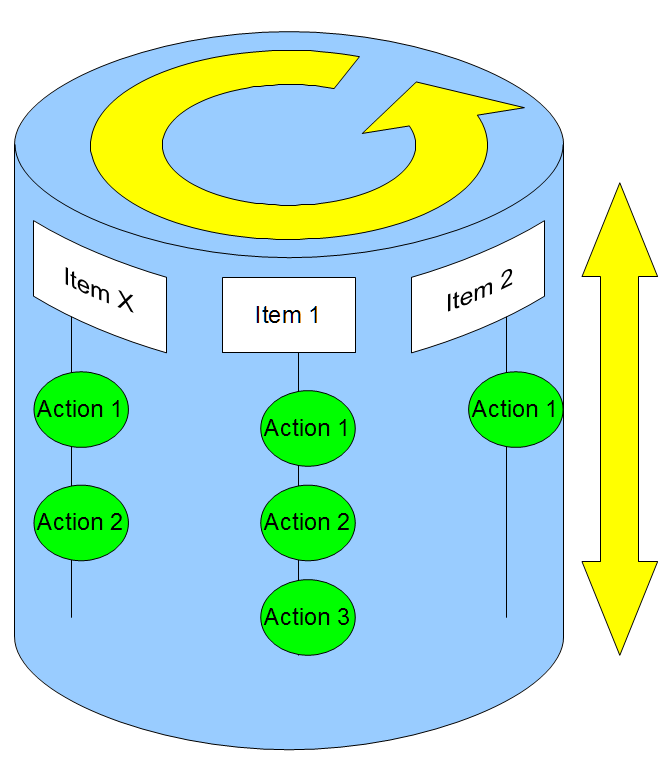
\includegraphics[width=0.5\linewidth]{computer.png}
\caption{Bracelet computer metaphor}
\label{draw}
\end{figure}
\section{Operation}
\subsection{Available actions}
\paragraph{}To keep users confident about using the computer, every kind of actions have the same meaning in all computer's items. It gives a consistency to the computer, and make easier the remembering of the how the computer works.
\begin{itemize}
\item \textbf{Left and Right Arrows} :  Allows to navigate between the items of the computer (going home, going to a particular place,...). 
\item \textbf{Up and Down arrows} : Allows navigation inside an item (switching current location display for example).
\item \textbf{Short push} : When you press the button less than 3 seconds. This action is most of the time a validation or a confirmation.
\item \textbf{Long push}  : A long is equivalent to holding the button for 3 seconds or more. It always brings you back to the screen that indicates the way home.
\end{itemize}
\paragraph{}The idea of having a long push allows one more action. The required pressed time might be discussed. It might maybe be part of settings, and be editable.The idea is to keep a permanent and easy access to the way home. 

\section{About functionalities}
\subsection{Current Location}
\paragraph{}This screen tells you were you are. Here is two displays : one (default) show you the street you are, and the other other one show you the nearest known place you are (Home or relatives house for example). When the place is indicated, we also provide the distance to that place.
\subsection{Going Home}
\paragraph{}We focused on keeping texts with graphics, when the screen size allows it. Direction is given by texts and arrows. In this computer, we try to minimize the use of graphics (only for directions). All the informations are given by text (even informations that appears on graphics). A directions changes is also follow by a vibration of the bracelet, to warn the user that he had to move.
\subsection{Going to a predefined place}
\paragraph{} When you're on that screen, the first thing to do is select a place. Thanks to the arrows, you can switch and select the place you want to go, then validate with a short push. Then the computer will give you indications on the way.
\subsection{Registered a new place}
\paragraph{}Users may need to add new places to the computer. As their is no keyboard, the solution we find is to have a predefined list of places that you can set (Home, supermarket, doctor, ...). To set a new location, users just have to be at that location, select it in the list, and validate.\\
Here, two cases can appears : 
\begin{enumerate}
\item \textbf{Location is free} : Computer allows you to set it.
\item \textbf{Location is already registered} : Computer will ask you a password, composed with arrows movements and validation, to avoid replacing an important location by mistake. 
\end{enumerate}

\subsection{Too far}
\paragraph{}The computer also provide a function to warn the user if is too far from the closest known place. The bracelet starts vibrate, and go to a special screen. From that screen, two ways to interact : Going to the closest known location, or going home. We use here some persuasion techniques (tunneling for that case), as the user can't choose anything else than those two choices.
\subsection{Maximum Distance}
\paragraph{}To enable the "Too far" function, the computer have to save a maximum allowed distance. This distance is editable. It's in meters (which is the unit for distance in the international system). We allow user to change that distance, but it required a password again (arrows + validation). Having this protection avoid user with dementia to modify it themselves. It the responsibility to people in charge to keep this password
\section*{Conclusion}
\paragraph{}This design is provided for elderly people, with dementia. The operations of the computer have been choose to be very simple, and based on Nielsen's principles (especially on graphics parts). Using the techniques we saw, we defined a design that help users, by avoiding mistakes and tunnel them on the good way on the computer, and in the real life !

%\bibliographystyle{plain}
%\bibliography{bib}

\end{document}